\documentclass[10pt,spanish,aspectratio=1610]{beamer}
\usepackage[utf8]{inputenc}
\usepackage{amsmath}
\usepackage{graphicx}
\usepackage{amssymb}
\usepackage[spanish]{babel}
\spanishdecimal{.}
\usepackage{subfig}
\usepackage{fancyhdr}
\usepackage{pstricks}
\usepackage{color}
\usepackage[ruled]{algorithm2e}
\usepackage{listings}
\usepackage{multicol}
\usepackage{xcolor}

\definecolor{graywhite}{rgb}{0.9529,0.9607,0.9686}
\definecolor{bluegray}{rgb}{0.6823, 0.7411, 0.8}
\definecolor{darkred}{rgb}{0.7372, 0.2392, 0.2392}
\definecolor{bluedark}{rgb}{0.294, 0.4705, 0.6407}
\definecolor{darkgreen}{rgb}{0.1764, 0.5294, 0.0901}
\lstset{
  backgroundcolor=\color{graywhite},   % choose the background color; you must add \usepackage{color} or \usepackage{xcolor}; should come as last argument
  basicstyle=\footnotesize,        % the size of the fonts that are used for the code
  breakatwhitespace=false,         % sets if automatic breaks should only happen at whitespace
  breaklines=true,                 % sets automatic line breaking
  captionpos=b,                    % sets the caption-position to bottom
  commentstyle=\color{darkgreen},    % comment style
  keepspaces=true,                 % keeps spaces in text, useful for keeping indentation of code (possibly needs columns=flexible)
  keywordstyle=\color{darkred},       % keyword style
  language=Octave,                 % the language of the code
  morekeywords={*,...},            % if you want to add more keywords to the set
  numbers=left,                    % where to put the line-numbers; possible values are (none, left, right)
  numbersep=7pt,                   % how far the line-numbers are from the code
  numberstyle=\tiny\color{bluedark}, % the style that is used for the line-numbers
  showspaces=false,                % show spaces everywhere adding particular underscores; it overrides 'showstringspaces'
  showstringspaces=false,          % underline spaces within strings only
  showtabs=false,                  % show tabs within strings adding particular underscores
  stepnumber=1,                    % the step between two line-numbers. If it's 1, each line will be numbered
  stringstyle=\color{bluedark},     % string literal style
  frame=single,
  rulecolor=\color{bluegray},
  tabsize=2,                   % sets default tabsize to 2 spaces
  xleftmargin=1cm,
  xrightmargin=0.5cm,
  framexleftmargin=0.5cm,
  extendedchars=true,
  literate={á}{{\'a}}1 {é}{{\'e}}1 {í}{{\'i}}1 {ó}{{\'o}}1 {ú}{{\'u}}1 {Á}{{\'A}}1 {É}{{\'E}}1 {Í}{{\'I}}1 {Ó}{{\'O}}1 {Ú}{{\'U}}1,
}

\DeclareMathOperator{\atantwo}{atan2}
\setbeamercolor{block title}{fg=white,bg=blue!70!black}
\setbeamercolor{block body}{fg=black, bg=blue!10!white}
\setbeamertemplate{blocks}[rounded][shadow=false]
\setbeamercovered{transparent}
\beamertemplatenavigationsymbolsempty
\setbeamertemplate{frametitle}{
  \leavevmode
  \hbox{\begin{beamercolorbox}[wd=0.6\paperwidth,left]{frametitle}
    \usebeamerfont{frametitle}\insertframetitle
  \end{beamercolorbox}
  \begin{beamercolorbox}[wd=0.4\paperwidth,center]{frametitle}
    \usebeamerfont{frametitle}\small{\thesection . \insertsectionhead}
  \end{beamercolorbox}  } }
\setbeamertemplate{footline}{
  \leavevmode%
  \hbox{%
    \begin{beamercolorbox}[colsep=-0.5pt,wd=.33\paperwidth,ht=3ex,dp=1.5ex,center]{author in head/foot}%
      \usebeamerfont{author in head/foot}\insertshortauthor~~ (\insertshortinstitute)
    \end{beamercolorbox}%
    \begin{beamercolorbox}[colsep=-0.5pt,wd=.34\paperwidth,ht=3ex,dp=1.5ex,center]{date in head/foot}%
      \usebeamerfont{author in head/foot}\insertshorttitle
    \end{beamercolorbox}%
    \begin{beamercolorbox}[colsep=-0.5pt,wd=.33\paperwidth,ht=3ex,dp=1.5ex,right]{author in head/foot}%
      \usebeamerfont{author in head/foot}\insertshortdate{} \hspace*{2em}\scriptsize{\insertframenumber{}}\hspace*{1ex}
    \end{beamercolorbox}
  }
}

\begin{document}
\renewcommand{\tablename}{Tabla}
\renewcommand{\figurename}{Figura}

\title[Tareas Básicas en Robots de Servicio Doméstico]{Tareas Básicas en Robots de Servicio Doméstico}
\author[Marco Negrete]{Instructor: Marco Antonio Negrete Villanueva}
\institute[FI, UNAM]{Facultad de Ingeniería, UNAM}
\date[EIR 2022]{Escuela de Invierno de Robótica 2022\\Modalidad a distancia\\\url{https://github.com/mnegretev/EIR-2022-AtHomeBasicTasks}}

\begin{frame}
\titlepage
\end{frame}

\begin{frame}\frametitle{Objetivos}
  \textbf{Objetivo General:} Brindar los conocimientos básicos necesarios para desarrollar un robot de servicio doméstico.
  \\
  \textbf{Objetivos Específicos:}
  \begin{itemize}
  \item Revisar el hardware necesario para tener un robot de servicio doméstico: sensores y actuadores más comunes.
  \item Dar un panorama general del software necesario para desarrollar un robot de servicio doméstico.
  \item Revisar las herramientas disponibles para cubrir las habilidades básicas requeridas en un robot de servicio doméstico:
    \begin{itemize}
    \item Navegación
    \item Vision
    \item Manipulación
    \item Síntesis y reconocimiento de voz
    \item Planeación de acciones
    %\item MoveIt (para manipulación de objetos)
    \end{itemize}
  \end{itemize}
\end{frame}

\begin{frame}\frametitle{Contenido}
  \tableofcontents
\end{frame}


\section{Introducción}

\begin{frame}
  \Huge
  Introducción
\end{frame}

\begin{frame}\frametitle{Los robots de servicio doméstico}
  \begin{columns}
    \begin{column}{0.5\textwidth}
      Son robots pensados para ayudar en tareas comunes del hogar u oficina. Requieren de varias habilidades:
      \begin{itemize}
      \item Interacción humano-robot
      \item Navegación en ambientes dinámicos
      \item Reconocimiento de objetos
      \item Manipulación de objetos
      \item Comportamientos adaptables
      \item Planeación de acciones
      \end{itemize}
    \end{column}
    \begin{column}{0.4\textwidth}
      \centering
      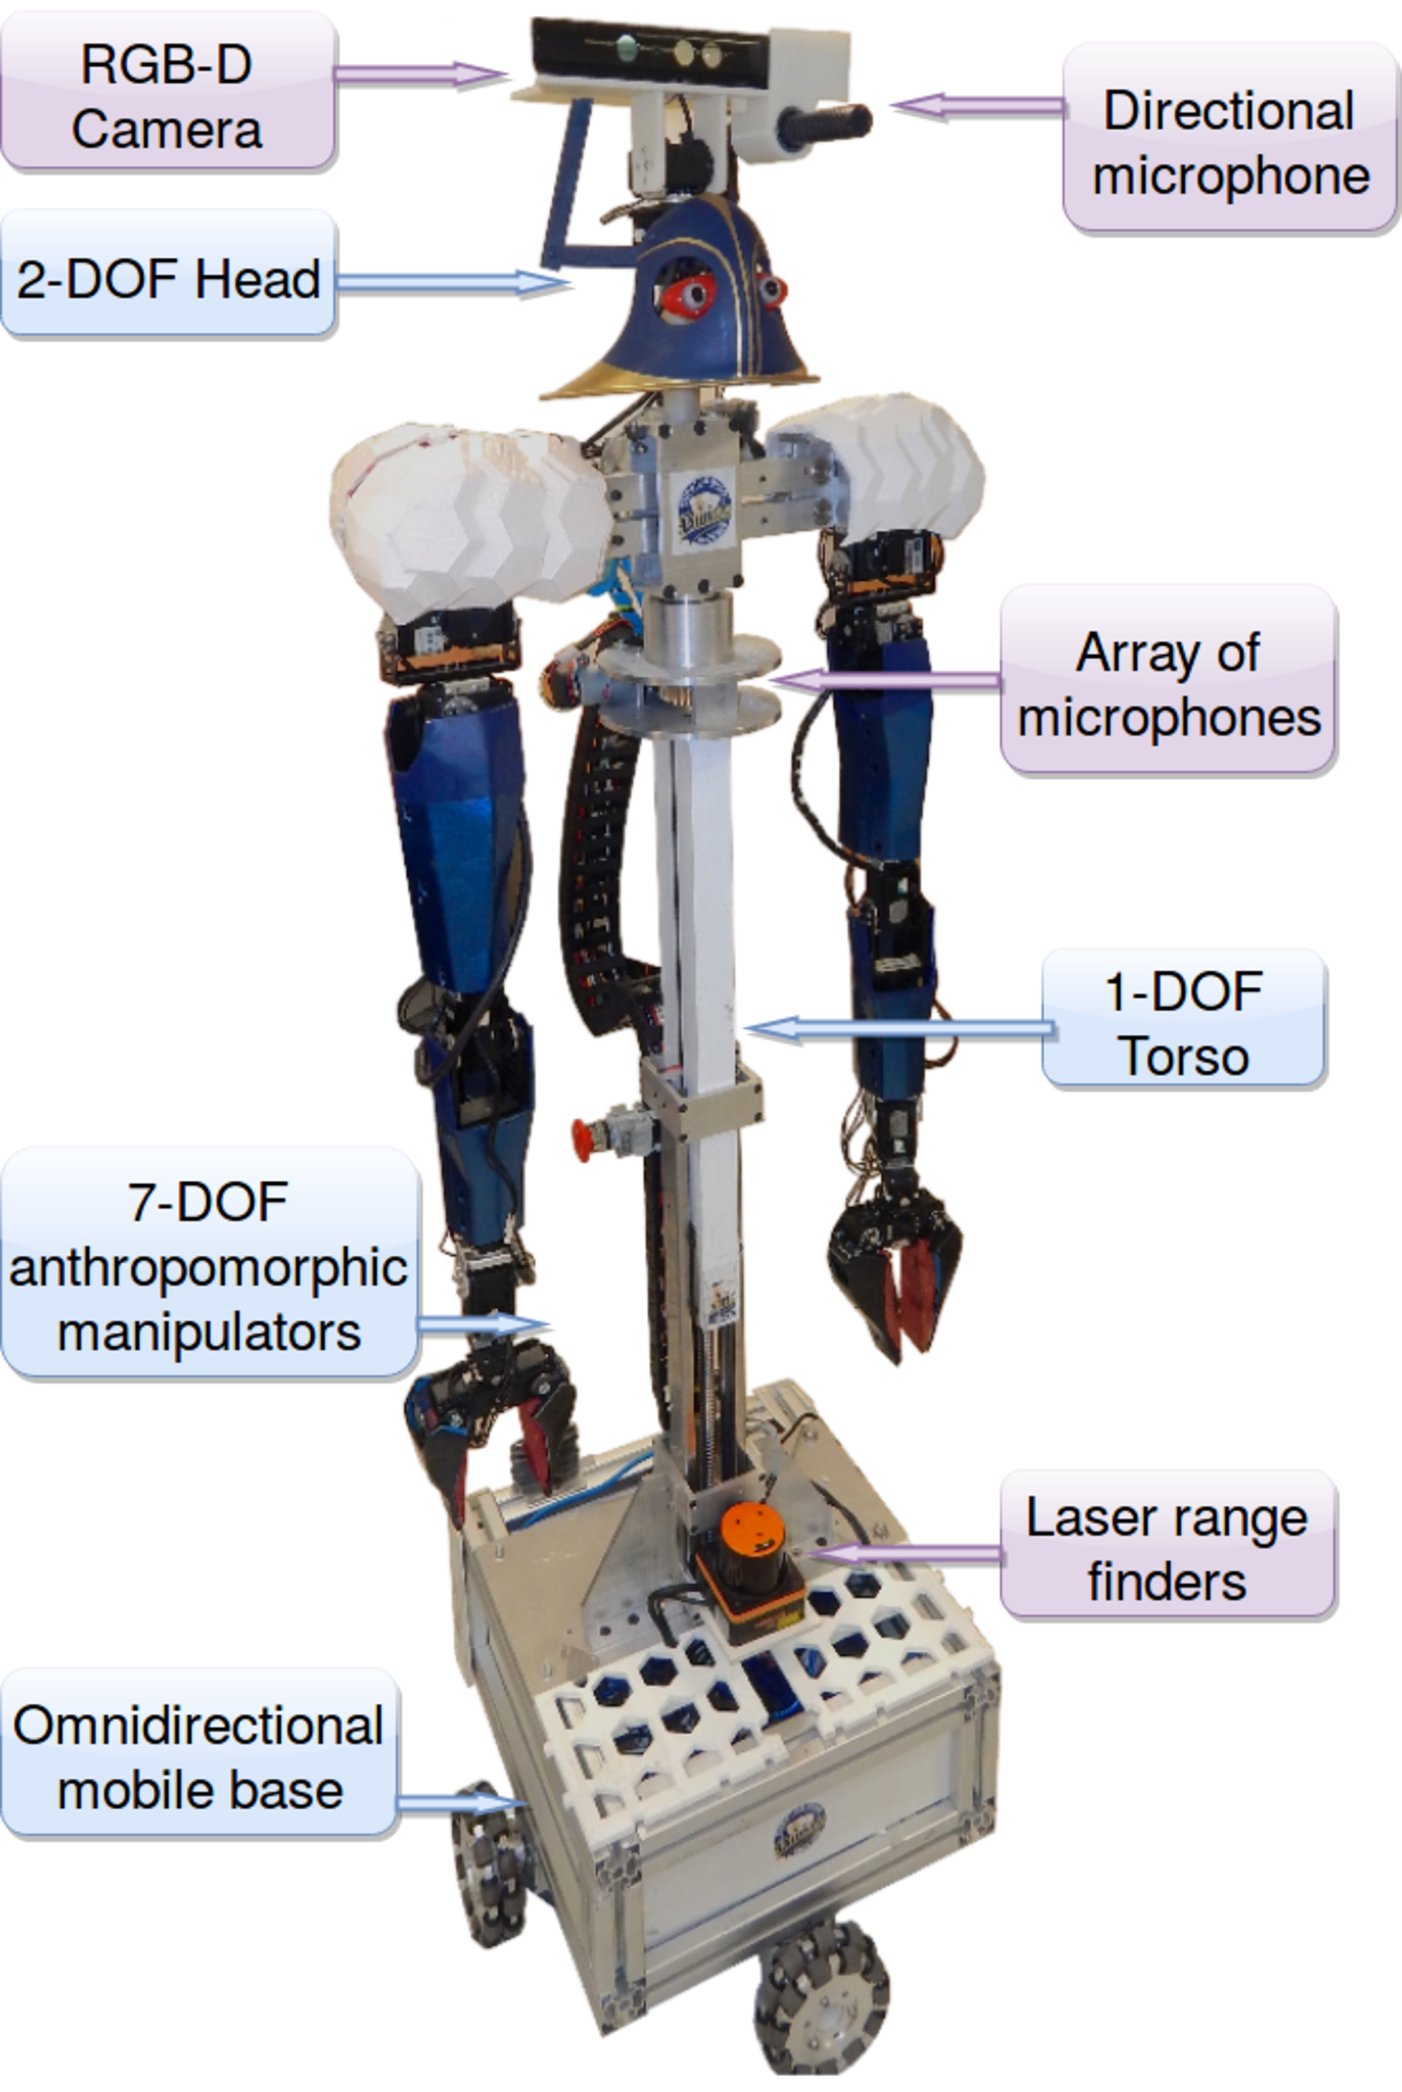
\includegraphics[width=0.9\textwidth]{Figures/Justina.pdf}
    \end{column}
  \end{columns}
\end{frame}

\begin{frame}\frametitle{Hardware necesario: Base móvil}
  \begin{columns}
    \begin{column}{0.5\textwidth}
      \begin{itemize}
      \item De preferencia, debe ser omnidireccional
      \item Turtle Bot (\url{https://www.turtlebot.com/})
      \item Festo Robotino (\url{https://wiki.openrobotino.org/})
      \item DIY: 3 ó 4 motores de corriente directa con ruedas omnidireccionales, 2 tarjetas Roboclaw, baterías de LiPo y chasis de alumnio estructural.
      \end{itemize}
    \end{column}
    \begin{column}{0.5\textwidth}
      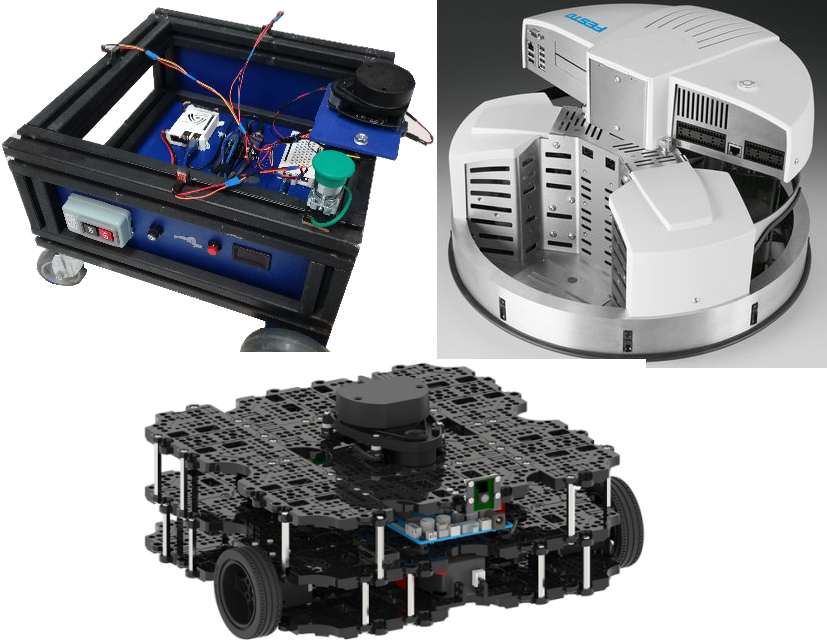
\includegraphics[width=\textwidth]{Figures/Bases.png}
    \end{column}
  \end{columns}
\end{frame}

\begin{frame}\frametitle{Hardware necesario: Cámaras}
  \begin{columns}
    \begin{column}{0.45\textwidth}
      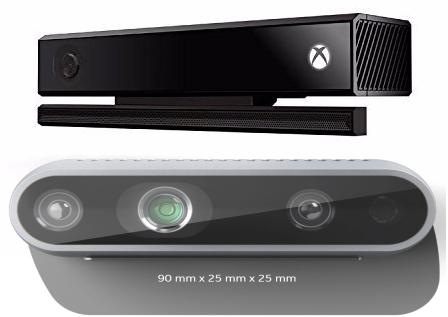
\includegraphics[width=\textwidth]{Figures/Cameras.jpg}
    \end{column}
    \begin{column}{0.5\textwidth}
      \begin{itemize}
      \item Se pueden usar sólo cámaras RGB, pero es altamente recomendable tener información de profundidad.
      \item Kinect (\url{https://github.com/OpenKinect/libfreenect2})
      \item Intel RealSense (\url{https://github.com/IntelRealSense/librealsense})
      \item También se pueden usar cámaras estéreo, pero es mucho más sencillo usar cámaras con luz estructurada.
      \end{itemize}
    \end{column}
  \end{columns}
\end{frame}

\begin{frame}\frametitle{Hardware necesario: Sensor láser}
  \begin{columns}
    \begin{column}{0.5\textwidth}
      \begin{itemize}
      \item Hokuyo (\url{https://www.hokuyo-aut.jp/})
      \item RPLidar (\url{https://www.robotshop.com/en/slamtec.html})
      \item SICK (\url{https://www.sick.com/ag/en/detection-and-ranging-solutions/2d-lidar-sensors/c/g91900})
      \item El paquete \url{http://wiki.ros.org/urg_node} facilita su operación.
      \item Si no se tiene uno, se puede simular a partir de una cámara RGB-D con el paquete \url{http://wiki.ros.org/pointcloud_to_laserscan}.
      \end{itemize}
    \end{column}
    \begin{column}{0.4\textwidth}
      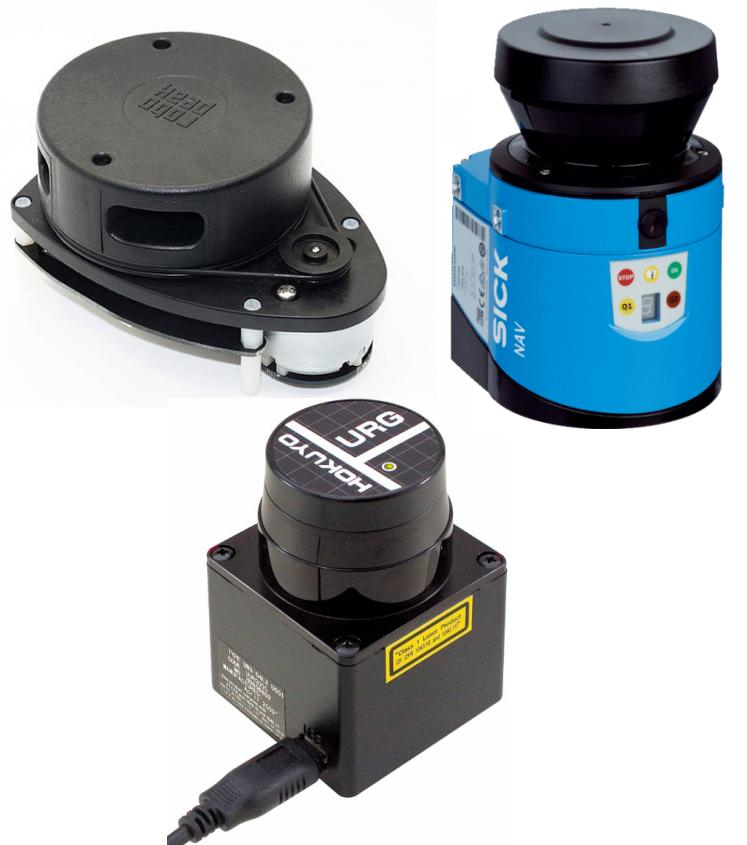
\includegraphics[width=\textwidth]{Figures/lasers.jpg}
    \end{column}
  \end{columns}
\end{frame}

\begin{frame}\frametitle{Hardware necesario: Manipulador}
  \begin{columns}
    \begin{column}{0.4\textwidth}
      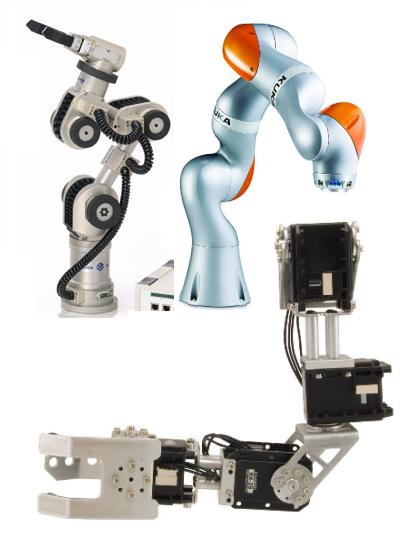
\includegraphics[width=\textwidth]{Figures/arms.jpg}
    \end{column}
    \begin{column}{0.5\textwidth}
      \begin{itemize}
      \item Son recomendables por lo menos 5 DOF.
      \item Kuka LBR iiwa (\url{http://wiki.ros.org/kuka})
      \item Neuronics Katana (\url{http://wiki.ros.org/katana})
      \item DIY: Servomotores y Brackets Dynamixel (\url{http://wiki.ros.org/dynamixel})
      \end{itemize}
    \end{column}
  \end{columns}
\end{frame}

\section{Conceptos Básicos}

\begin{frame}
  \Huge
  Conceptos básicos
\end{frame}

\begin{frame}\frametitle{Funciones comunes}
  \textbf{Sigmoide}: Es una función que puede ser usada como una versión \textit{suave} del escalón. Se usará en en control de posición y en el entrenamiento de redes neuronales.
  \[\sigma(x) = \frac{1}{1 + e^{-x}}\]
  La derivada tiene la forma:
  \[\frac{d\sigma}{dx}=\frac{-(-e^{-x})}{\left(1 + e^{-x}\right)^2} = \frac{1 + e^{-x} - 1}{\left(1 + e^{-x}\right)^2}=\frac{1}{1+e^{-x}}\left(1 - \frac{1}{1 + e^{-x}}\right) = \sigma(x)(1 - \sigma(x))\]
  \textbf{Campana de Gauss}: Es una función siempre positiva que tiende a cero cuando $|x|\rightarrow \infty$:
  \[f(x) = a \cdot e^{-\frac{(x - b)^2}{2c^2}}\]
\end{frame}

\begin{frame}\frametitle{Gradiente}
  Dada una función $f:\mathbb{R}^n \rightarrow \mathbb{R}$, es decir, una función escalar de variable vectorial $f(x_1, x_2, \dots, x_n)$, el gradiente $\nabla f(\bar{x})$ está dado por:
  \[\nabla f(\bar{x}) = \left[ \frac{\partial f}{\partial x_1}, \frac{\partial f}{\partial x_2}, \dots \frac{\partial f}{\partial x_n}\right]^T\]

  \begin{itemize}
  \item El gradiente generaliza el concepto de derivada para funciones de varias variables.
  \item El gradiente evaluado en un punto $\bar{x}_0$ indica la dirección de máximo cambio en ese punto.
  \end{itemize}
\end{frame}

\begin{frame}\frametitle{Jacobiano}
  Dada una función $F:\mathbb{R}^n \rightarrow \mathbb{R}^m$, es decir, una función vectorial de variable vectorial:
  \[F(\bar{x}) = \begin{tabular}{l}$f_1(x_1, x_2, ..., x_n)$\\$f_2(x_1, x_2, ..., x_n)$\\ $\vdots$ \\ $f_n(x_1, x_2, ..., x_n)$\end{tabular}\]
  El Jacobiano es una matriz que contiene las primeras derivadas parciales:
  \[J(x) = \left[\begin{tabular}{cccc}
      $\dfrac{\partial f_1}{\partial x_1}$ & $\dfrac{\partial f_1}{\partial x_2}$ & $\dots$ & $\dfrac{\partial f_1}{\partial x_n}$\\
      & & &\\
      $\dfrac{\partial f_2}{\partial x_1}$ & $\dfrac{\partial f_2}{\partial x_2}$ & $\dots$ & $\dfrac{\partial f_2}{\partial x_n}$\\
      & $\vdots$ & & \\
      $\dfrac{\partial f_m}{\partial x_1}$ & $\dfrac{\partial f_m}{\partial x_2}$ & $\dots$ & $\dfrac{\partial f_m}{\partial x_n}$\\
    \end{tabular}\right] = \left[\begin{tabular}{c}$\nabla^T f_1$\\ $\nabla^T f_2$ \\ $\vdots$ \\ $\nabla^T f_m$\end{tabular}\right]\in\mathbb{R}^{m\times n}\]
\end{frame}

\begin{frame}\frametitle{Espacio de Configuraciones}
  La \textit{configuración} de un robot (o de una parte de él) es una descripción de todos los puntos que ocupa en el espacio. Los \textit{grados de libertad} son el conjunto mínimo de valores independientes que se requieren para definir una configuración.
  \[\]
  La configuración de un cuerpo rígido que se mueve en el espacio tiene 6 grados de libertad (tres para posición y tres para orientación): $(x,y,z,\psi,\theta,\phi)$. Si el cuerpo se mueve sólo en el plano, tiene 3 grados: $(x,y,\theta)$ (una posición en 2D y una orientación).
\end{frame}


\section[Navegación]{Navegación}

\begin{frame}
  \Huge
  Navegación
\end{frame}

\begin{frame}\frametitle{Planeación de movimientos}
  El problema de la planeación de movimientos comprende cuatro tareas básicas:
  \begin{itemize}
  \item Navegación (encontrar una ruta por el espacio libre de un punto inicial a uno final). Si la ruta está parametrizada con repecto al tiempo, se dice que es una trayectoria.
  \item Mapeo (construir una representación del ambiente a partir de las lecturas de los sensores y la configuración)
  \item Localización (determinar la configuración a partir de un mapa y de lecturas de los sensores)
  \item Barrido (pasar un actuador por todos los puntos de un subespacio)
  \end{itemize}
  Comúnmente el mapeo y la localización se realizan al mismo tiempo en el proceso conocido como SLAM (\textit{Simultaneous Localization and Mapping})
\end{frame}

\begin{frame}\frametitle{Celdas de ocupación}
  Es una discretización del espacio con una resolución determinada donde a cada celda se le asigna un número $p\in[0,1]$ que indica su nivel de ocupación.
  \begin{itemize}
  \item En un enfoque probabilístico, $p$ indica la certeza de que la celda esté ocupada: 0, certeza de que está libre, 1, certeza de que está ocupada, 0.5, no se tiene información.
  \item En este curso, los niveles de ocupación solo serán 0 o 1.
 Para evitar el manejo de flotantes, el nivel de ocupación suele representarse con un entero en el intervalo [0,100] y un -1 si no hay información. 
  \end{itemize}
  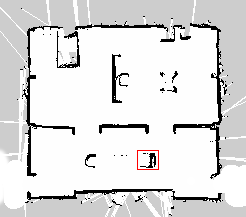
\includegraphics[width=0.4\textwidth]{Figures/OccupancyGrid.png}
  
\includegraphics[width=0.4\textwidth]{Figures/OccupancyGridZoom.png}
\end{frame}

\begin{frame}[containsverbatim]\frametitle{Ejercicio 1}
  Ejecute el comando:
  \begin{lstlisting}
    roslaunch bring_up path_planning.launch
  \end{lstlisting}
  Inspeccione el mapa en el visualizador RViz. Luego abra el archivo:
  \texttt{catkin\_ws/src/config\_files/maps/appartment.pgm}
  con cualquier editor de imágenes y modifíquelo.
  \\Detenga la ejecución y vuelva a correr el comando anterior. 
\end{frame}

\begin{frame}\frametitle{Planeación de rutas}
  Dado un espacio de configuraciones $Q$ con espacio libre $Q_{free}\subset Q$ y espacio ocupado $Q_{occ}\subset Q$, la planeación de rutas consiste en contrar un mapeo:
  \[f: [0,1] \rightarrow Q_{free} \qquad \textrm{con}\qquad f(0) = q_s\qquad f(1)=q_g\]
  donde $q_s$ y $q_g$ son las configuraciones inicial y meta, respectivamente. Es decir, se debe encontrar una secuencia de puntos del espacio libre que permitan al robot moverse del punto inicial al punto meta sin chocar. Los métodos para planear rutas se pueden agrupar en:
  \begin{itemize}
  \item Basados en búsqueda en grafos (A*, Dijkstra)
    \begin{itemize}
    \item En un mapa de celdas de ocupación, cada celda libre es un nodo del grafo.
    \item Cada nodo está conectado con las celdas vecinas del espacio libre. 
    \end{itemize}
  \item Basados en muestreo (RRT)
  \item Variacionales
  \end{itemize}
\end{frame}

\begin{frame}\frametitle{El algoritmo A*}
    \begin{algorithm}[H]
    \footnotesize
    \DontPrintSemicolon
    \KwData {Mapa $M$ de celdas de ocupación, configuración inicial $q_{start}$, configuración meta $q_{goal}$}
    \KwResult{Ruta $P=[q_{start},q_1, q_2, \dots , q_{goal}]$}
    \;
    Obtener los nodos $n_s$ y $n_g$ correspondientes a $q_{start}$ y $q_{goal}$\;
    Lista abierta $OL = \emptyset$ y lista cerrada $CL = \emptyset$\;
    \ForAll{Nodo $n \in M$}
    {
      $g(n) = \infty \qquad f(n) = \infty$\;
    }
    Agregar $n_s$ a $OL$\;
    $g(n_s) = 0 \qquad f(n_s) = 0$\;
    Nodo actual $n_c = n_s$\;
    \While{$OL\neq \emptyset$ y $n_c\neq n_g$}
    {
      Seleccionar de $OL$ el nodo $n_c$ con el menor valor $f$ y agregar $n_c$ a $CL$\;
      \ForAll{Vecino $n$ de $n_c$}
      {
        Calcular los valores $g$ y $h$ para el nodo $n$\;
        \If{$g < g(n)$}
        {
          $g(n) = g\qquad f(n) = g + h \qquad Previo(n) = n_c$
        }
      }
      Agregar a $OL$ los vecinos de $n_c$ que no estén ya en $OL$ ni en $CL$\;
    }
    \If{$n_c\neq n_g$}{Anunciar Falla}
    Obtener la configuración $q_i$ para cada nodo $n_i$ de la ruta\;
  \end{algorithm}
\end{frame}

\begin{frame}\frametitle{El algoritmo A*}
  El valor $g$ es una función de costo y el algoritmo A* siempre devolverá la ruta que minimice el costo total del nodo inicial al nodo meta. Las funciones más comunes son:
  \begin{itemize}
  \item Distancia de Manhattan: $d(p_1, p_2) = |p_{1_x} - p_{2_x}| + |p_{1_y} - p_{2_y}|$
  \item Distancia Euclidiana: $d(p_1, p_2) = \left( (p_{1_x} - p_{2_x})^2 + (p_{1_y} - p_{2_y})^2 \right)^{1/2}$
  \end{itemize}
  En la función $g$ se puede incluir cualquier criterio para planear una ruta: la más corta, la más rápida, la más segura, etc.\\
  La heurística $h$ sirve para expandir menos nodos y es una función que debe \textit{subestimar} el costo real de llegar de un nodo $n$ al nodo meta $n_g$. La distancia Euclidiana y la distancia de Manhattan son dos funciones también muy usadas como heurísticas. 
\end{frame}

\begin{frame}[containsverbatim]\frametitle{Ejercicio 2}
  Ejecute el comando:
  \begin{lstlisting}
    roslaunch bring_up path_planning.launch
  \end{lstlisting}
  En otra terminal, ejecute el comando:
  \begin{lstlisting}
    rosrun exercises a_star.py
  \end{lstlisting}
  Utilizando la GUI calcule una ruta desde la posición del robot hasta el punto (0,0). En el visualizador \texttt{RViz} se mostrará la ruta calculada.\\
  \begin{figure}
    \centering
    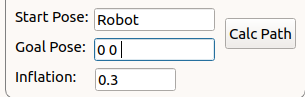
\includegraphics[width=0.35\textwidth]{Figures/Exercise1Gui.png}
    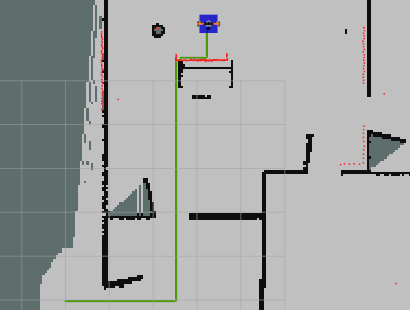
\includegraphics[width=0.35\textwidth]{Figures/Exercise1Rviz.png}
  \end{figure}
\end{frame}

\begin{frame}[containsverbatim]\frametitle{Ejercicio 2}
  Detenga la ejecución del programa \texttt{a\_star.py}. \\
    Modifique el archivo \texttt{catkin\_ws/src/exercises/scripts/a\_star.py} para utilizar distancia Euclidiana en lugar de distancia de Manhattan. Modifique las secciones marcadas con el comentario \texttt{\#Ejercicio}. 
    \lstinputlisting[language=Python,firstnumber=26]{Codes/AStar1.py}
    \lstinputlisting[language=Python,firstnumber=49]{Codes/AStar2.py}
    Ejecute nuevamente el comando
    \begin{lstlisting}
    rosrun exercises a_star.py
    \end{lstlisting}
    Y compare los resultados. 
\end{frame}

\begin{frame}\frametitle{Inflado de mapas}
  Para evitar que se calculen rutas por espacios por donde el robot en realidad no puede pasar debido a sus dimensiones, los obstáculos del mapa se deben \textit{inflar} cuando menos un número de celdas igual al radio del robot.\\
  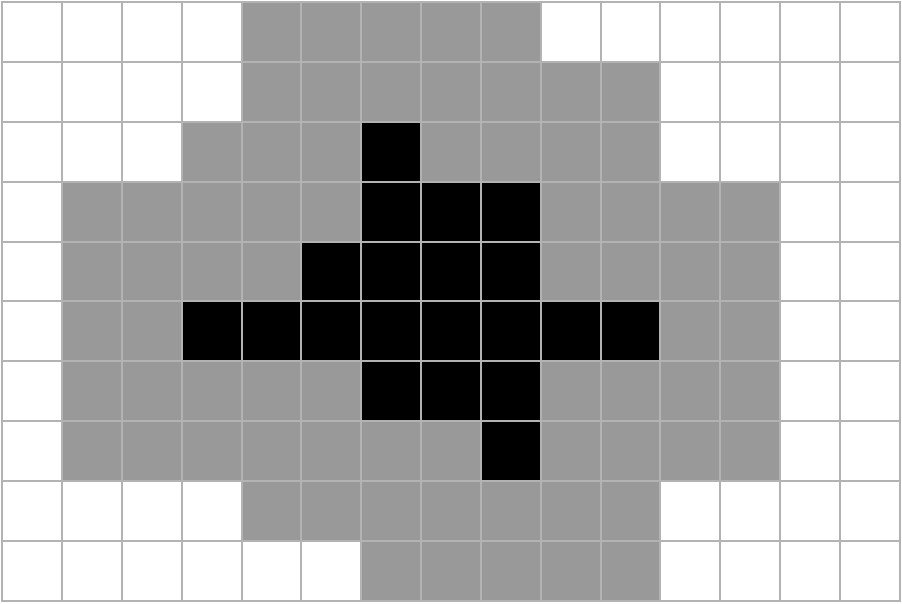
\includegraphics[width=0.45\textwidth]{Figures/Inflation.pdf}
  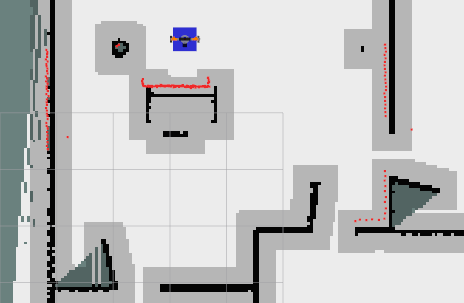
\includegraphics[width=0.45\textwidth]{Figures/Inflation.png}
\end{frame}

\begin{frame}[containsverbatim]\frametitle{Ejercicio 3}
  Modifique el archivo \texttt{catkin\_ws/src/exercises/scripts/inflation.py} para implementar el algoritmo de inflado de obstáculos:
  \lstinputlisting[language=Python,firstnumber=19]{Codes/Inflation.py}
  Ejecute el comando:
  \begin{lstlisting}
    roslaunch bring_up path_planning.launch
  \end{lstlisting}
  En otra terminal, ejecute el comando:
  \begin{lstlisting}
    rosrun exercises a_star.py
  \end{lstlisting}
  Y en una tercera terminal ejecute el comando
  \begin{lstlisting}
    rosrun exercises inflation.py
  \end{lstlisting}
\end{frame}

\begin{frame}\frametitle{Control de posición}
  Suponiendo que el robot está en la posición y orientación $(x,y, \theta)$ y que se quiere alcanzar la posición deseada $(x_g, y_g)$, como se muestra en la figura. Las leyes de control
  \begin{multicols}{2}
    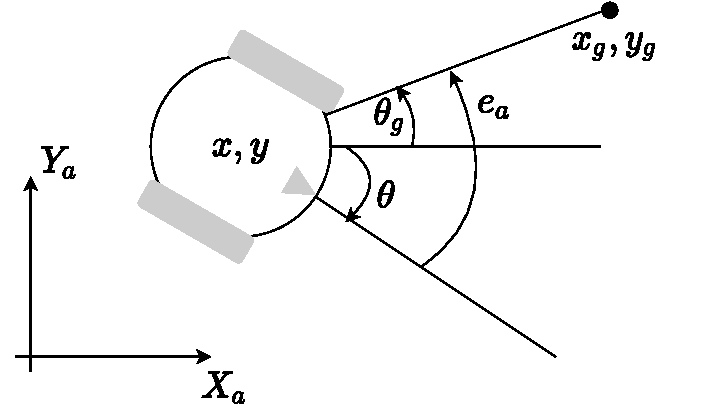
\includegraphics[width=0.5\textwidth]{Figures/GoalPose.pdf}
    \[\]
  \begin{eqnarray*}
    v &=& v_{max} e^{-e_a^2/\alpha}\\
    \omega &=& \omega_{max}\left(\frac{2}{1 + e^{-e_a/\beta}} - 1\right)
  \end{eqnarray*}
  \end{multicols}
  con $e_a = \textrm{atan2}(y_g - y, x_g - x) - \theta$, permiten que el robot alcance la posición deseada. Los parámetros $v_{max}$ y $\omega_{max}$ se deben seleccionar de acuerdo con las capacidades del robot. Las constantes $\alpha$ y $\beta$ permiten controlar qué tan rápido cambian la velocidad lineal y angular del robot. 
\end{frame}


\begin{frame}\frametitle{Seguimiento de rutas}
  El control de posición se puede utilizar para seguir una ruta si se fija como punto meta cada punto de la ruta, hasta alcanzar el último.
  \begin{figure}
    \centering
    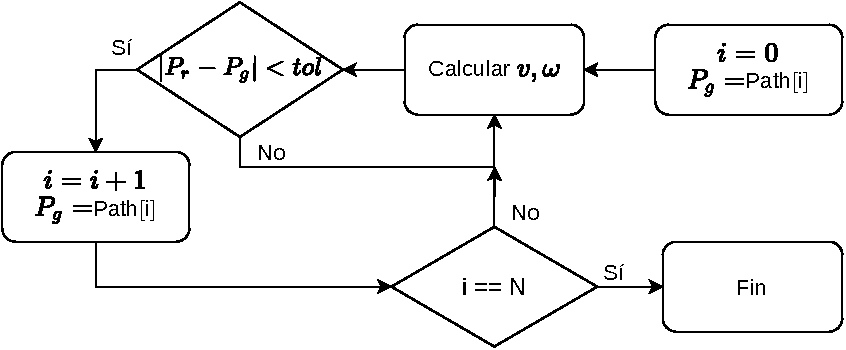
\includegraphics[width=0.6\textwidth]{Figures/PathFollowing.pdf}
  \end{figure}
\end{frame}


\begin{frame}[containsverbatim]\frametitle{Ejercicio 4}
  Ejecute el comando:
  \begin{lstlisting}
    roslaunch bring_up path_planning.launch
  \end{lstlisting}
  En otra terminal, ejecute el comando:
  \begin{lstlisting}
    roslaunch bring_up exercises_path_planning.launch
  \end{lstlisting}
  Utilizando RViz, envíe el robot a un punto meta:
  \begin{figure}
    \centering
    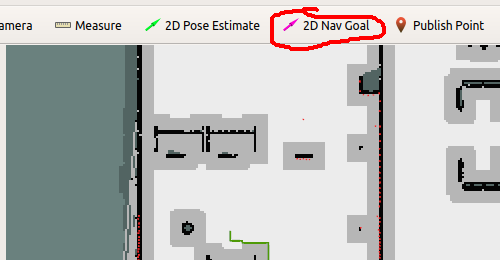
\includegraphics[width=0.5\textwidth]{Figures/Exercise4Rviz.png}
  \end{figure}
\end{frame}

\begin{frame}[containsverbatim]\frametitle{Ejercicio 4}
  Detenga la ejecución de los ejercicios. Abra el archivo \texttt{catkin\_ws/src/exercises/scripts/control.py} y modifique las constantes $v_{max}$, $\omega_{max}$, $\alpha$ y $\beta$.
  \lstinputlisting[language=Python,firstnumber=23]{Codes/Control.py}
  Vuelva a ejecutar el comando
  \begin{lstlisting}
    roslaunch bring_up exercises_path_planning.launch
  \end{lstlisting}
  Y compare el comportamiento del robot.
\end{frame}

\section{Visión}
\begin{frame}\frametitle{Las imágenes como funciones}
  
\end{frame}

\begin{frame}\frametitle{Espacios de color}
  
\end{frame}

\begin{frame}\frametitle{Histograma de color}
\end{frame}

\begin{frame}\frametitle{Nubes de puntos}
  
\end{frame}

\begin{frame}\frametitle{Extracción de planos}
  
\end{frame}


\begin{frame}\frametitle{Agrupamiento}
  
\end{frame}

\begin{frame}\frametitle{Ejercicio}
Quitar plano de la mesa y reconocer por color.   
\end{frame}

\begin{frame}\frametitle{Redes neuronales}
  
\end{frame}


\begin{frame}\frametitle{Ejercicio}
  
\end{frame}


\section{Manipulación}

\begin{frame}\frametitle{Posición y Orientación}
  Un cuerpo rígido en el espacio puede tener una posición $(x,y,z)$ y una orientación. La orientación se puede representar de varias formas:
  \begin{itemize}
  \item Mediante ángulos de Euler: roll, pich y yaw $RPY = (\psi, \theta, \phi)$
  \item Mediante cuaterniones
  \item Mediante una matriz de rotación $R \in SO(3)$
  \end{itemize}
  Los ángulos $RPY$ son rotaciones intrínsecas sobre los ejes $X$, $Y$, y $Z$ respectivamente. Se llaman intrínsecas porque son rotaciones que ocurren sobre un sistema de referencia \textit{atado} a un cuerpo rígido.\\
  Cualquier orientación se puede obtener mediante la composición de tres rotaciones básicas:
  \[R = R_{z,\phi}R_{y,\theta}R_{x,\psi}\]
  Es decir, primero una rotación de $\phi$ radianes sobre el eje $Z$, seguida de una rotación de $\theta$ radianes sobre el eje $Y$ del sistema resultante y una rotación de $\psi$ radianes sobre el eje $X$ del sistema rotado. 
\end{frame}

\begin{frame}\frametitle{Transformaciones Homogéneas}
  Una Transformación Homogénea es una matriz de la forma
  \[T = \left[\begin{tabular}{cccc}
      & & & $d_x$\\
      & $R\in SO(3)$ & & $d_y$\\
      & & & $d_z$\\
      0 & 0& 0 & 1
    \end{tabular}\right]\]
  Puede servir para
  \begin{itemize}
  \item Representar la posición y orientación de un cuerpo rígido
  \item Representar una transformación de coordenadas $T_{ab}$ de un sistema de referencia $b$ a un sistema $a$
  \end{itemize}
  Propiedades:
  \begin{itemize}
  \item Asociatividad: $(T_1 T_2) T_3 = T_1 (T_2 T_3)$
  \item Inversa:
    \[T = \left[\begin{tabular}{cc}
       $R^T$ & $-R^T d$\\
       0 & 1
      \end{tabular}\right]\]
  \item Cancelación de índices: $T_{ab} = T_{ac}T_{cb}$
  \end{itemize}
\end{frame}

\begin{frame}\frametitle{El árbol cinemático}
  Es útil tener una descripción de la forma en que están conectadas las diferentes articulaciones del robot. Se considera que sobre cada articulación hay un sistema de referencia (\textit{frame}) que está trasladado y rotado con respecto al sistema anterior.
  \begin{multicols}{3}
    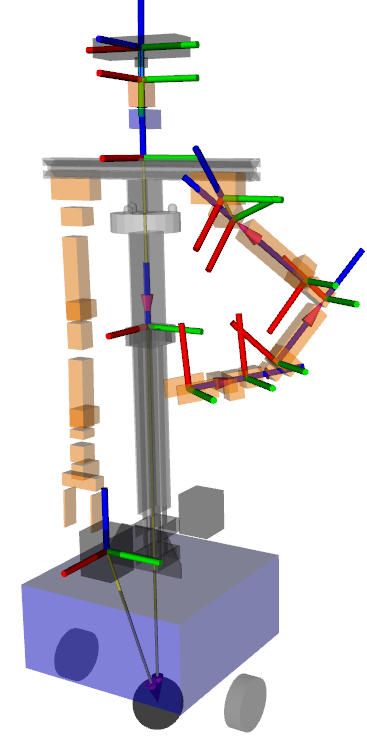
\includegraphics[width=0.26\textwidth]{Figures/KinematicTree.png}\\
    \footnotesize
    El sistema \textit{absoluto} se suele llamar \texttt{map}\\
    El sistema base del robot se suele llamar \textit{base\_link}\\
    Las transformaciones de \texttt{map} a \texttt{base\_link} las determina el sistema de localización\\
    El resto de las transformaciones se determinan con la posición de cada articulación\\
    El árbol cinemático se traduce en una cadena de mulplicaciones de Transformaciones Homogéneas. 
    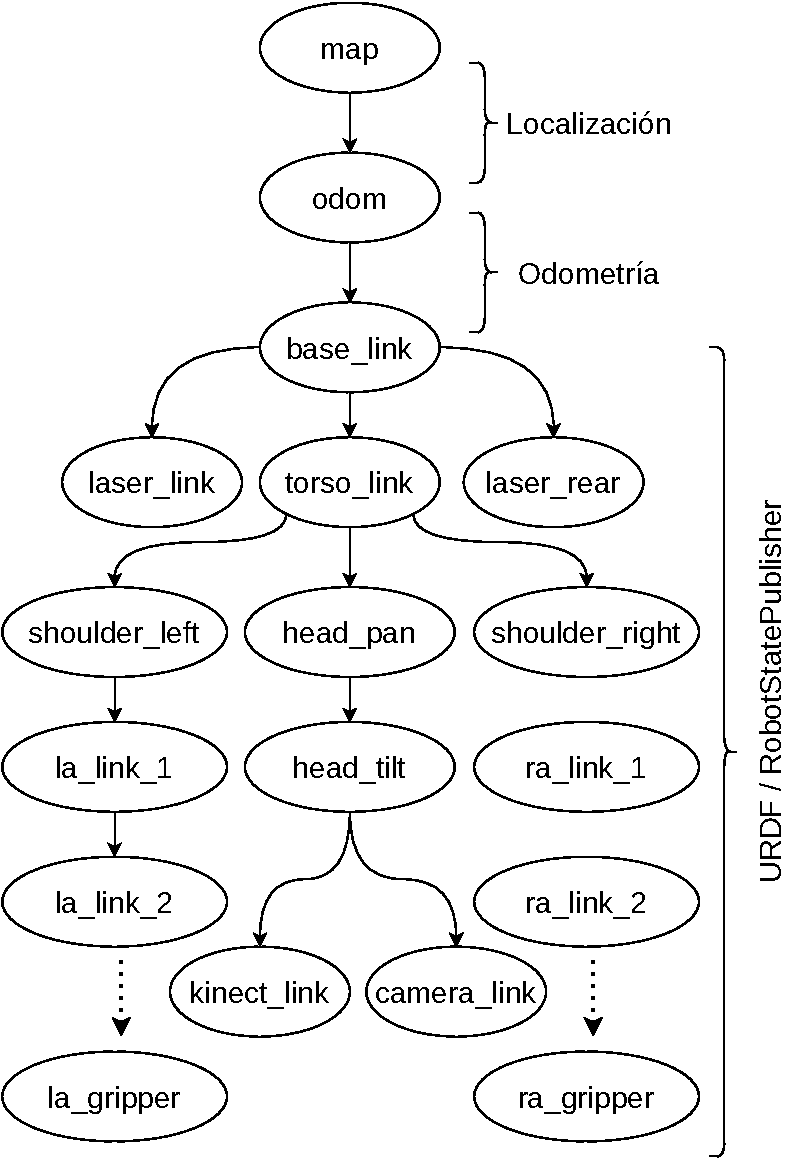
\includegraphics[width=0.35\textwidth]{Figures/TfTree.pdf}
  \end{multicols}
\end{frame}

\begin{frame}[containsverbatim]\frametitle{El formato URDF}
  El formato URDF permite describir el arbol cinemático del robot mediante etiquetas XML:
  \footnotesize
  \lstinputlisting[language=XML]{Codes/URDFExample.xml}
  \normalsize
  Cada etiqueta \texttt{<joint>} representará una Transformación Homogénea. 
\end{frame}

\begin{frame}[containsverbatim]\frametitle{El formato Xacro}
  El formato Xacro es un lenguaje de \textit{macros} que permite obtener archivos XML más cortos. Es últil para especificar parámetros físicos en el URDF como inercias y volúmenes:
  \footnotesize
  \lstinputlisting[language=XML]{Codes/XacroExample.xml}
\end{frame}

\begin{frame}[containsverbatim]\frametitle{Ejercicio}
  Abra el archivo \texttt{catkin\_ws/src/hardware/justina\_description/urdf/justina\_base.xacro} y vaya a la línea 228:
  \lstinputlisting[language=XML,firstnumber=227]{Codes/JustinaXacro.xml}
  Modifique el atributo \texttt{xyz} y aumente 1 m en la coordenada en z. Después ejecute el comando:
  \begin{lstlisting}
    roslaunch bring_up path_planning.launch
  \end{lstlisting}
  Detenga la simulación. Ahora modifique el atributo \texttt{rpy}, cambie los valores a ``1.5708 0 0'' y ejecute de nuevo la simulación. 
\end{frame}

\begin{frame}\frametitle{La cinemática directa}
  La cinemática directa consiste en determinar la posición y orientación del efector final del manipulador a partir de la posición de cada articulación.  Esta se puede calcular con la ecuación:
  \[P_1 = T_{12}T_{23}T_{34}T_{45}T_{56}T_{67}T_{7g}P_g\]
  donde $P_g = [0,0,0,1]^T$ es la posición del gripper con respecto al sistema del gripper, $P_1$ es la posición del gripper con respecto al sistema base y $T_{ab}$ es la transformación homogénea que define la rotación y traslación producida por cada articulación. Las matrices $T_{ab}$
  tienen la forma:
  \[T_{ab} = \left[\begin{tabular}{cccc}
      & & & $dx_{ab}$\\
      & $R_{ab}\in SO(3)$ & & $dy_{ab}$\\
      & & & $dz_{ab}$\\
      0 & 0& 0 & 1
    \end{tabular}\right]\]
  Donde $R_{ab}$ representa la rotación del sistema $b$ respecto al sistema $a$ y $(dx_{ab}, dy_{ab}, dz_{ab})$ es la traslación del sistema $b$ respecto al sistema $a$.\\
  La rotación $R_{ab}$ está definida en el URDF por el atributo ``rpy'' de la sub etiqueta \texttt{origin} de la etiqueta \texttt{joint} y por la posición de la articulación. La traslación $(dx_{ab}, dy_{ab}, dz_{ab})$ está definida por el atributo ``xyz''. 
\end{frame}

\begin{frame}\frametitle{Ejercicio}
  Abra el archivo ... y modifique las líneas ...
\end{frame}

\begin{frame}\frametitle{La cinemática inversa}
  La cinemática inversa consiste en determinar las posiciones que debe tener cada articulación para que el efector final tenga la posición y orientación deseadas.
  \begin{itemize}
  \item Mientras la cinemática directa siempre tiene solución, la cinemática inversa, no.
  \item Se puede resolver por métodos geométricos para obtener una solución cerrada, aunque el análisis puede ser muy complicado.
  \item Una solución más general se puede obtener mediante un método numérico. 
  \end{itemize}
  Suponiendo que se tiene una configuración deseada $p_d \in \mathbb{R}^6$ ($xyz-RPY$), se desea encontrar el conjunto de posiciones articulares $q\in\mathbb{R}^7$ que satisfagan la ecuación
  \[FK(q) - p_d = 0\]
  donde la función $FK$ representa la cinemática directa. 
\end{frame}

\begin{frame}\frametitle{El método Newton-Raphson}
  El método numérico de Newton-Raphson sirve para encontrar raíces, es decir, para resolver ecuaciones de la forma
  \[f(x) = 0\]
  El algoritmo es el siguiente:
  \[\]
  \begin{multicols}{2}
  \begin{algorithm}[H]
    \DontPrintSemicolon
    $x_i \leftarrow x_0$\;
    \While{$|f(x)| > \epsilon$}
    {
       $x_{i+1} \leftarrow x_i - \frac{f(x_i)}{f'(x_i)}$
    }
  \end{algorithm}
  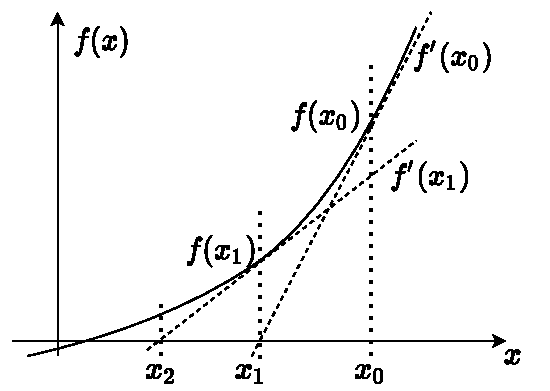
\includegraphics[width=0.4\textwidth]{Figures/NewtonRaphson.pdf}
  \end{multicols}
\end{frame}

\begin{frame}\frametitle{El Jacobiano}
  El Jacobiano es una matriz que relaciona la velocidad articular $\dot{q}$ con la velocidad en el espacio cartesiano $[v\;\omega]^T$ (velocidad lineal y angular):
  \[\dot{p} = \left[\begin{tabular}{c}$v$\\$\omega$\end{tabular}\right] = J \dot{q}
  \qquad\qquad p = [x,y,z,roll, pitch, yaw] \in \mathbb{R}^6, \quad J\in \mathbb{R}^{6\times 7},\quad q\in \mathbb{R}^7\]
  \[J = \left[ \begin{tabular}{ccc}
      $\frac{\partial p_1}{\partial q_1}$ & $\cdots$ & $\frac{\partial p_1}{\partial q_7}$\\
      $\vdots$ & $\ddots$ & $\vdots$ \\
      $\frac{\partial p_6}{\partial q_1}$ & $\cdots$ & $\frac{\partial p_6}{\partial q_7}$\\
    \end{tabular} \right]\]
  \begin{itemize}
  \item La matriz $J$ se puede obtener analíticamente, sin embargo, dado el número de grados de libertad, resulta muy complicado
  \item Se puede obtener aproximando las derivadas parciales con diferencias finitas:
  \end{itemize}
  \[J = \left[\frac{FK(q^1_{+}) -  FK(q^1_{-})}{2\Delta q} \qquad \cdots \qquad \frac{FK(q^7_{+}) -  FK(q^7_{-})}{2\Delta q}\right]\]
  \begin{eqnarray*}
    q^i_+ &=& [q_1\quad \dots \quad q_i + \Delta q \quad \dots \quad q_7]\\
    q^i_- &=& [q_1\quad \dots \quad q_i - \Delta q \quad \dots \quad q_7]
  \end{eqnarray*}
  con $\Delta q$, un valor lo suficientemente pequeño para una buena aproximación de la derivada. 
\end{frame}

\begin{frame}\frametitle{Cinemática Inversa por Newton-Raphson}
  Aplicando Newton-Raphson para resolver la ecuación:
  \[FK(q) - p_d = 0\]
  Se tiene:
  \begin{algorithm}[H]
    \DontPrintSemicolon
    $q_i \leftarrow q_0$ //Una estimación inicial que puede ser la posición articular actual\;
    $p \leftarrow FK(q_i)$ //La posición cartesiana que tendría el gripper con la estimación inicial\;
    \While{$|p - p_d| > \epsilon$}
    {
      $J \leftarrow Jacobiano(q)$     \;
      $q_{i+1} \leftarrow q_i - J^\dagger (p - p_d)$\;
      $p \leftarrow FK(q_i)$ 
    }
  \end{algorithm}
  Puesto que el Jacobiano $J$ no es una matriz cuadrada, no tiene inversa, por lo que se utiliza la matriz pseudoinversa $J^\dagger$. 
  \begin{itemize}
  \item Es importante que las variables angulares siempre estén en el intervalo $(-\pi, \pi]$:
    \begin{itemize}
    \item Las posiciones articulares
    \item Los ángulos roll, pitch, yaw
    \item Las componentes angulares del error $p - p_d$
    \end{itemize}
  \end{itemize}
\end{frame}

\begin{frame}\frametitle{El control PID}
  El control Proporcional-Integral-Derivativo es un tipo de control lineal en lazo cerrado que calcula la acción de control mediante una combinación lineal del error, la integral del error y la derivada del error.
  \begin{itemize}
  \item Para el manipulador, el ángulo deseado $q_d$ está dado por el resultado de la cinemática inversa. 
  \item La posición angular $q$ se obtiene de los motores o del simulador.
  \item La salida del controlador es el torque $\tau$ que se envía a los motores.
  \end{itemize}
  En la versión continua:
  \[\tau(t) = K_p e(t) + K_I \int e(t)dt + K_d \dot{e}(t)\]
  con $e = q_d - q$
  En la versión discreta:
  \[\tau_i = K_p e_i + K_I\sum_{j=0}^i e_j + K_d\frac{e_i - e_{i-1}}{\Delta t}\]
  con $\Delta t$, el periodo de muestreo. 
\end{frame}

\begin{frame}\frametitle{Los \textit{stacks} ros\_control y ros\_controllers}
  Es un conjunto de paquetes que implementa controladores PID y varias interfaces de hardware.
  \begin{itemize}
  \item El paquete \texttt{controller\_manager} utilizar un archivo \textit{yaml} para lanzar otros nodos que implementan controladores. 
  \item El paquete \texttt{joint}
  \end{itemize}
\end{frame}

\begin{frame}\frametitle{Ejercicio}
  Abra el archivo \texttt{justina\_controllers.yaml} y modifique las ganancias de las articulaciones. Detenga la simulación y ejecútela de nuevo para ver qué sucede. 
\end{frame}

\section{Síntesis de Voz}

\begin{frame}\frametitle{Síntesis de voz con SoundPlay}
  \begin{itemize}
  \item Es un paquete que permite reproducir archivos \texttt{.wav} o \texttt{.ogg}, sonidos predeterminados y síntesis de voz.
  \item La síntesis de voz se hace utilizando Festival (\url{http://www.cstr.ed.ac.uk/projects/festival/}).
  \item Para sintetizar voz, basta con correr el nodo \texttt{soundplay\_node} y publicar un mensaje de tipo \texttt{sound\_play/SoundRequest} con lo siguiente:
    \begin{itemize}
    \item msg\_speech.sound   = -3                 
    \item msg\_speech.command = 1                  
    \item msg\_speech.volume  = 1.0                
    \item msg\_speech.arg2    = ``voz a utilizar''
    \item msg\_speech.arg = ``texto a sintetizar''
    \end{itemize}
  \end{itemize}
\end{frame}

\begin{frame}[containsverbatim]\frametitle{Ejercicio 9}
  Ejecute el comando:
  \begin{lstlisting}
    roslaunch bring_up speech_synthesis.launch
  \end{lstlisting}
  En otra terminal, ejecute el comando:
  \begin{lstlisting}
    rosrun exercises speech_synthesis.py "my first synthetized voice"
  \end{lstlisting}
  Para instalar más voces:
  \begin{itemize}
  \item Ejecute el comando \texttt{sudo apt-get install festvox-<voz deseada>}
  \item Para ver qué voces se tienen instaladas: \texttt{ls /usr/share/festival/voices/english/}
  \end{itemize}
\end{frame}

\begin{frame}[containsverbatim]\frametitle{Ejercicio 9}
  Modifique el archivo \texttt{catkin\_ws/src/exercises/scripts/speech\_synthesis.py} y cambie la voz a utilizar en el mensaje SoundRequest.
  \lstinputlisting[language=Python,firstnumber=17]{Codes/SpeechSynthesis.py}
  El nombre de la voz se compone de \texttt{voice\_} más el nombre que aparece en la carpeta \texttt{/usr/share/festival/voices/english/}. 
\end{frame}

\section{Reconocimiento de voz}
\begin{frame}\frametitle{Reconocimiento de voz con Pocketsphinx}
  Pocketsphinx es un \textit{toolkit} open source desarrollado por la Universidad de Carnegie Mellon (\url{https://cmusphinx.github.io/}).
  \begin{itemize}
  \item Aunque el toolbox original no está hecho específicamente para ROS, ya existen varios repositorios con nodos ya implementados que integran ROS y Pocketsphinx:
    \begin{itemize}
    \item \url{https://github.com/mikeferguson/pocketsphinx}
    \item \url{https://github.com/Pankaj-Baranwal/pocketsphinx}
    \end{itemize}
  \item El usuario debe estar agregado al grupo \textit{audio} para el correcto funcionamiento: \texttt{sudo usermod -a -G audio <user\_name>}
  \end{itemize}
  \begin{itemize}
  \item Se puede hacer reconocimiento usando una lista de palabras, un modelo de lenguaje o una gramática.
  \item Se utilizarán gramáticas y sus correspondientes diccionarios.
  \item Para construir diccionarios, visitar \url{https://cmusphinx.github.io/wiki/tutorialdict/}
  \item Para construir gramáticas, visitar \url{https://www.w3.org/TR/2000/NOTE-jsgf-20000605/}
  \end{itemize}
\end{frame}

\begin{frame}\frametitle{Ejercicio 10}
  \begin{enumerate}
  \item Verifique el volumne del micrófono
  \item Inspeccione el archivo \texttt{catkin\_ws/src/pocketsphinx/vocab/gpsr.gram} para ver las frases que se pueden reconocer de acuerdo con la gramática.
  \item Ejecute el comando \texttt{roslaunch bring\_up speech\_recognition.launch}
  \item En otra terminal, ejecute el comanto \texttt{rostopic echo /recognized}
  \item Pruebe el reconocimiento de voz con alguna de las siguientes frases:
    \begin{enumerate}
    \item \texttt{Robot, take the pringles to the table}
    \item \texttt{Robot, take the drink to the table}
    \item \texttt{Robot, take the pringles to the kitchen}
    \item \texttt{Robot, take the drink to the kitchen}
    \end{enumerate}
  \end{enumerate}
\end{frame}

\section{Planeación de acciones}

\begin{frame}
  \Huge
  Planeación de acciones
\end{frame}

\begin{frame}\frametitle{Máquinas de estados finitas}
  Las FSM son modelos que permiten representar procesos discretos donde el sistema puede estar en un estado bien definido y existen un conjunto de reglas para definir el estado siguiente en función del estado actual y las entradas. Opcionalmente, se pueden definir salidas para cada estado. \\
  Formalmente, una FSM está definida por:
  \begin{itemize}
  \item $S$ : Conjunto finito no vacío de estados
  \item $\Sigma$ : Conjunto finito no vacío de entradas
  \item $s_0 \in S$ : Estado inicial
  \item $\delta : S\times\Sigma\rightarrow S$ : Función de transición de estados
  \item $F$ : Conjunto de estados finales (puede ser un conjunto vacío)
  \end{itemize}
\end{frame}

\begin{frame}\frametitle{Carta ASM}
  Una forma de representar los estados y transiciones de una FSM es mediante una carta ASM. Ejemplo:
  \begin{figure}
    \centering
    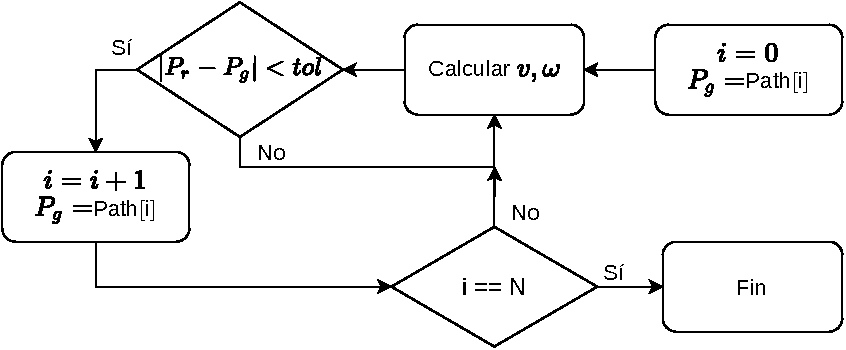
\includegraphics[width=0.6\textwidth]{Figures/PathFollowing.pdf}
  \end{figure}
  Las máquinas de estados se pueden utiizar para ejecutar tareas ``sencillas'' en un robot de servicio doméstico. 
\end{frame}


\bibliographystyle{abbrv}
\bibliography{References}
\end{document}
